This chapter is dedicated to the exposition and analysis of our experimental results. We shall commence by showcasing the performance of our model, meticulously comparing it against the baseline model derived from preceding work. The comparison will span across two crucial stages - the generation of weak labels and the ultimate segmentation performance.

Beyond the comparative assessment, we thrust into the realm of statistical validation using the t-test. This step solidifies our evidence by testing the hypothesis concerning the improvement observed in our results.

Through this dual approach, with a comparative study augmented by rigorous statistical validation, we aim to furnish a comprehensive demonstration of capabilities and advancements of our model over existing methods. Collectively, these analyses form the backbone of our arguments, underpinning the significant contribution of our work in advancing the state-of-the-art in segmentation tasks.

\section{Weak Label generation}

A crucial component of our training pipeline is the process of weak label generation. This stage, marked by the utilization of centerline coordinates for creating a preliminary weak mask and subsequent enhancement through training with limited fully-connected data, plays a pivotal role in determining the final segmentation model performance.

With an emphasis on the decisive influence of the quality of weak labels, we present an in-depth comparison of performance of our approach against the baseline model (Table \ref{tab:mask-generation-comparison}). The results are examined in terms of the Dice Similarity Coefficient (DSC), with the details presented using the format \(\mu_i \pm \sigma_{i}\), where \(\mu\) and \(\sigma\) denote the mean and variance of the DSC on test instances respectively.

\begin{table}[ht]
    \begin{subtable}[b]{\textwidth}
        \centering
        \begin{tabular}{c | c | c}
        Model & Average DSC (Axial) & Average DSC (Coronal) \\
        \hline
        Baseline & \(0.5553 \pm 0.0755\)  & \(0.5463 \pm 0.0986\)\\
        \hline
        Our Method & \(\mathbf{0.8084 \pm 0.0695}\) & \(\mathbf{0.6941 \pm 0.0871}\) 
       \end{tabular}
       \caption{Average Case Comparison}
       \label{tab:average-mask-generation}
    \end{subtable}
    \vfill
    \begin{subtable}[b]{\textwidth}
        \centering
        \begin{tabular}{c | c | c}
        Model & Best DSC (Axial) & Best DSC (Coronal) \\
        \hline
        Baseline & 0.6305 & 0.6559\\
        \hline
        Our Method & \(\mathbf{0.8843}\) & \(\mathbf{0.8251}\)
       \end{tabular}
       \caption{Best Case Comparison}
       \label{tab:best-mask-generation}
    \end{subtable}
     \caption{Weak Lable Generation Comparison}
     \label{tab:mask-generation-comparison}
\end{table}

In both the average and best-case scenarios, our method exhibits an appreciable edge over the baseline in terms of DSC values for axial and coronal images as shown in Tables \ref{tab:average-mask-generation} and \ref{tab:best-mask-generation}. It is noteworthy to highlight that our approach significantly outperforms the baseline derived from preceding work \cite{Ali2022}. In terms of average performance, we observe uplifts of 45.58\% and 11.97\% for Axial T2 and Coronal images respectively.

The sizable improvement is also evident when examining the best performance for each case type. With a remarkable increase of 40.24\% for Axial T2 and a substantial 25.8\% rise for Coronal T2 images, our approach convincingly demonstrates its effectiveness.

These results underline the efficacy of our method in generating high-quality weak labels that substantially enhance the final segmentation performance. These findings offer a promising perspective on the potential of our strategy to contribute meaningfully to advancements in terminal ileum segmentation tasks.

\subsection{Visual Validation of Model Performance}
We offer a graphical representation of our models performance in Figure \ref{fig:comparison-mask-gt}, providing a direct comparison between the generated weak masks and the corresponding ground truth annotations across both Coronal and Axial modalities.

Upon detailed observation, one can notice that the weak masks generated by our model align significantly well with the ground truth, as evidenced by the regions coloured yellow which represent either the ground truth segmentation or the generated mask.

As portrayed in the paired images (Figs. \ref{fig:gt-axial} and \ref{fig:mask-axial} for Axial T2; Figs. \ref{fig:gt-coronal} and \ref{fig:mask-coronal} for Coronal T2), the substantial overlaps between our generated mask and the ground truth are noteworthy, with hardly discernible discrepancies.

This visual illustration accentuates the robustness of our model in generating highly accurate weak masks, thereby mirroring closely the ground truth. Consequently, our model demonstrates remarkable potential in facilitating precise and dependable terminal ileum segmentation tasks, bridging the gap between machine-generated weak masks and human-annotated ground truths.

\begin{figure}[htp]
    \centering
    \begin{subfigure}[b]{0.48\textwidth}
        \centering
        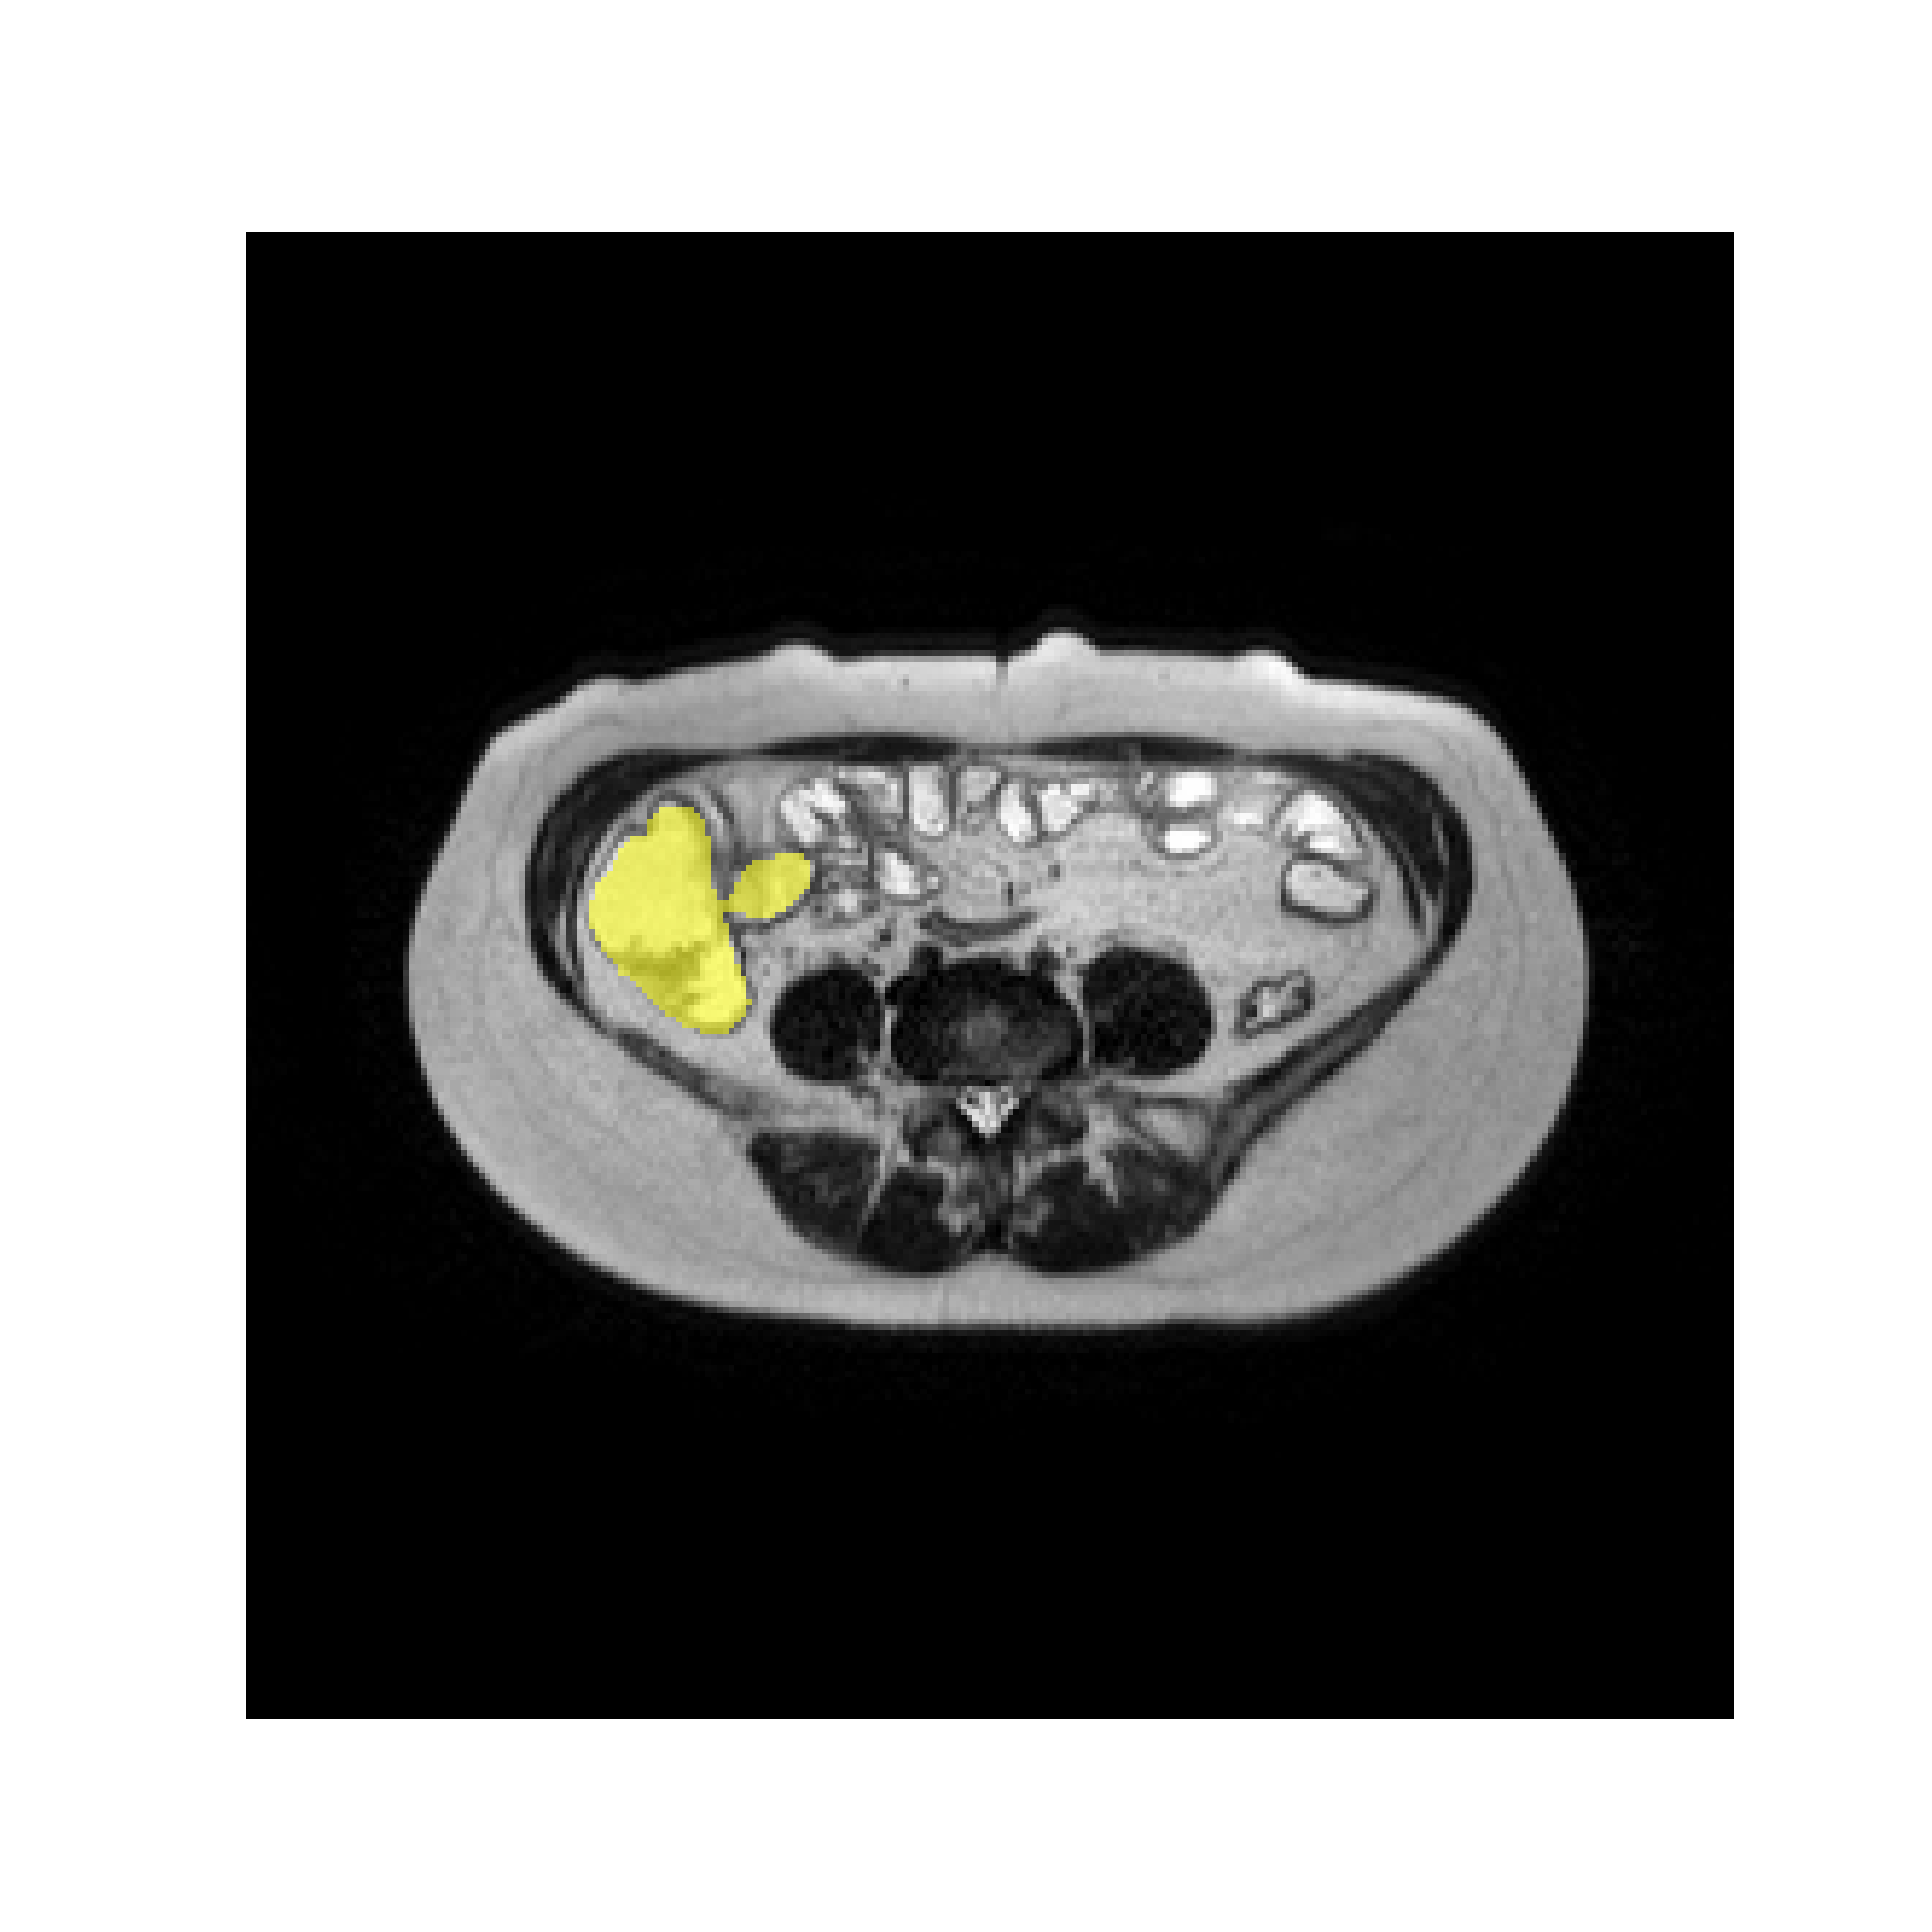
\includegraphics[width=\textwidth]{./figures/weak_mask_axial_gt.png}
        \caption{Ground Truth on Axial T2}
        \label{fig:gt-axial}
    \end{subfigure}
    \hfill
    \begin{subfigure}[b]{0.48\textwidth}
        \centering
        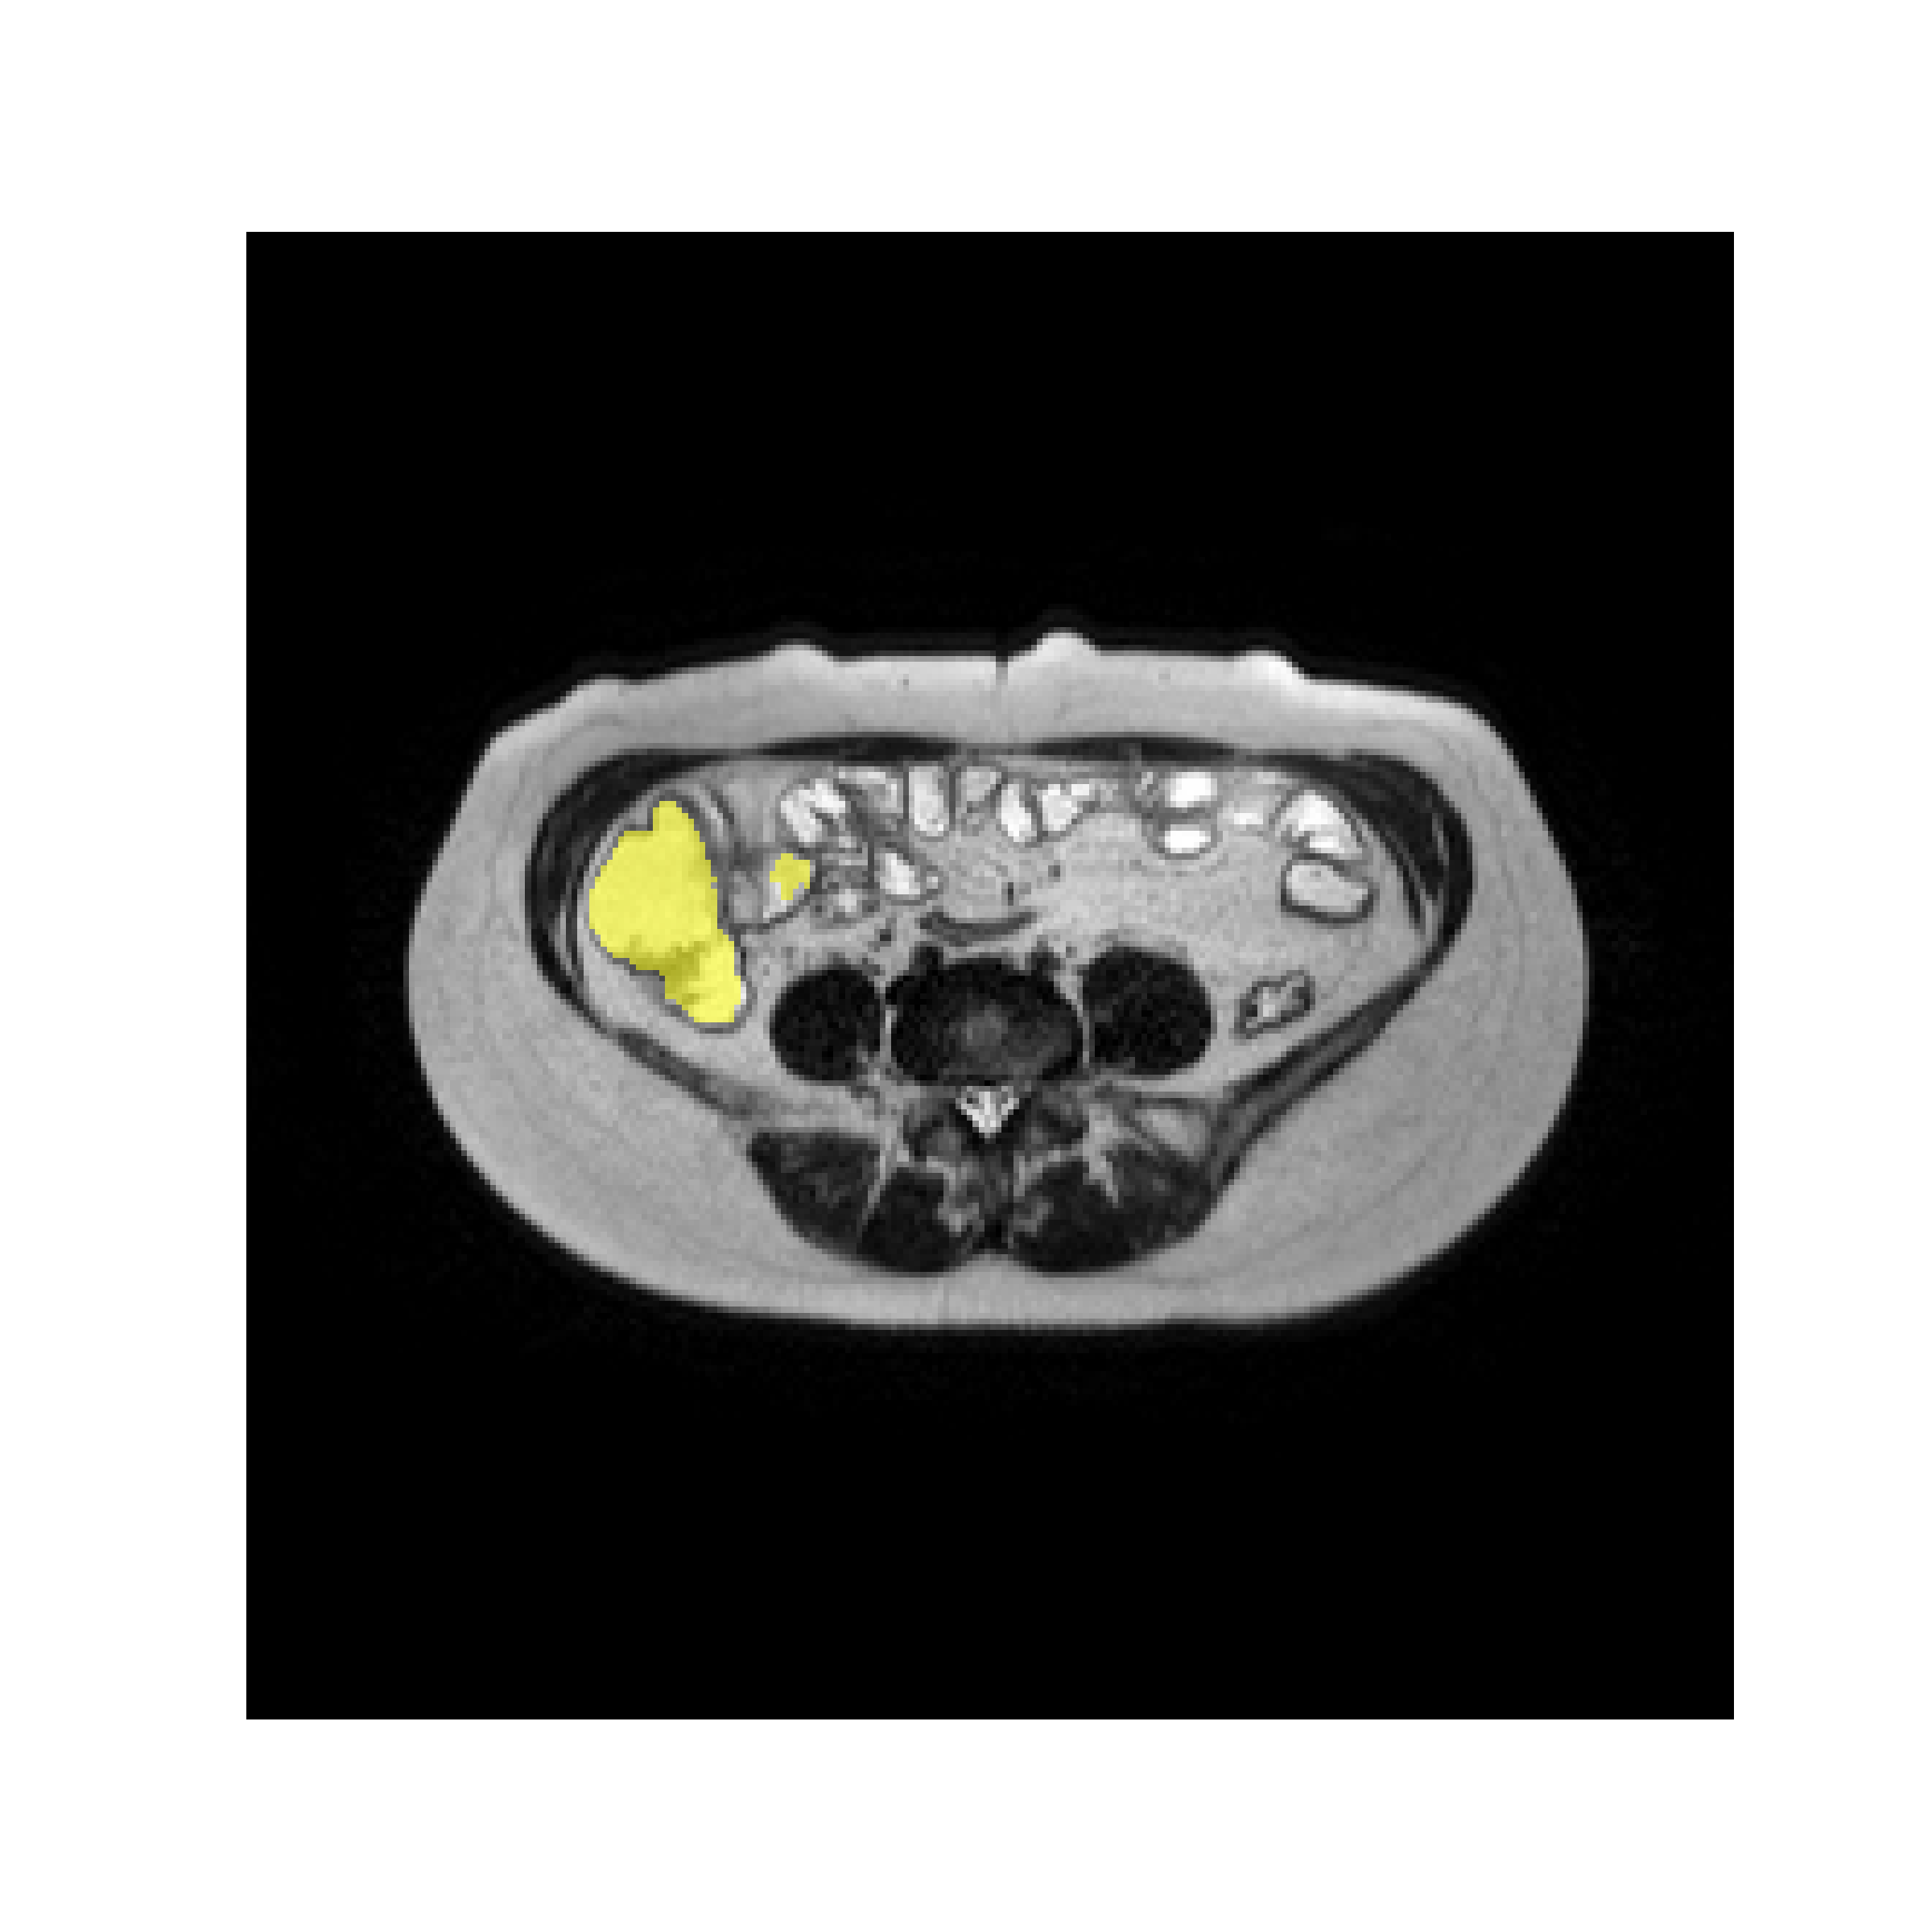
\includegraphics[width=\textwidth]{./figures/weak_mask_axial_medsam.png}
        \caption{Weak Mask on Axial T2}
        \label{fig:mask-axial}
    \end{subfigure}
    \vskip\baselineskip
    \begin{subfigure}[b]{0.48\textwidth}
        \centering
        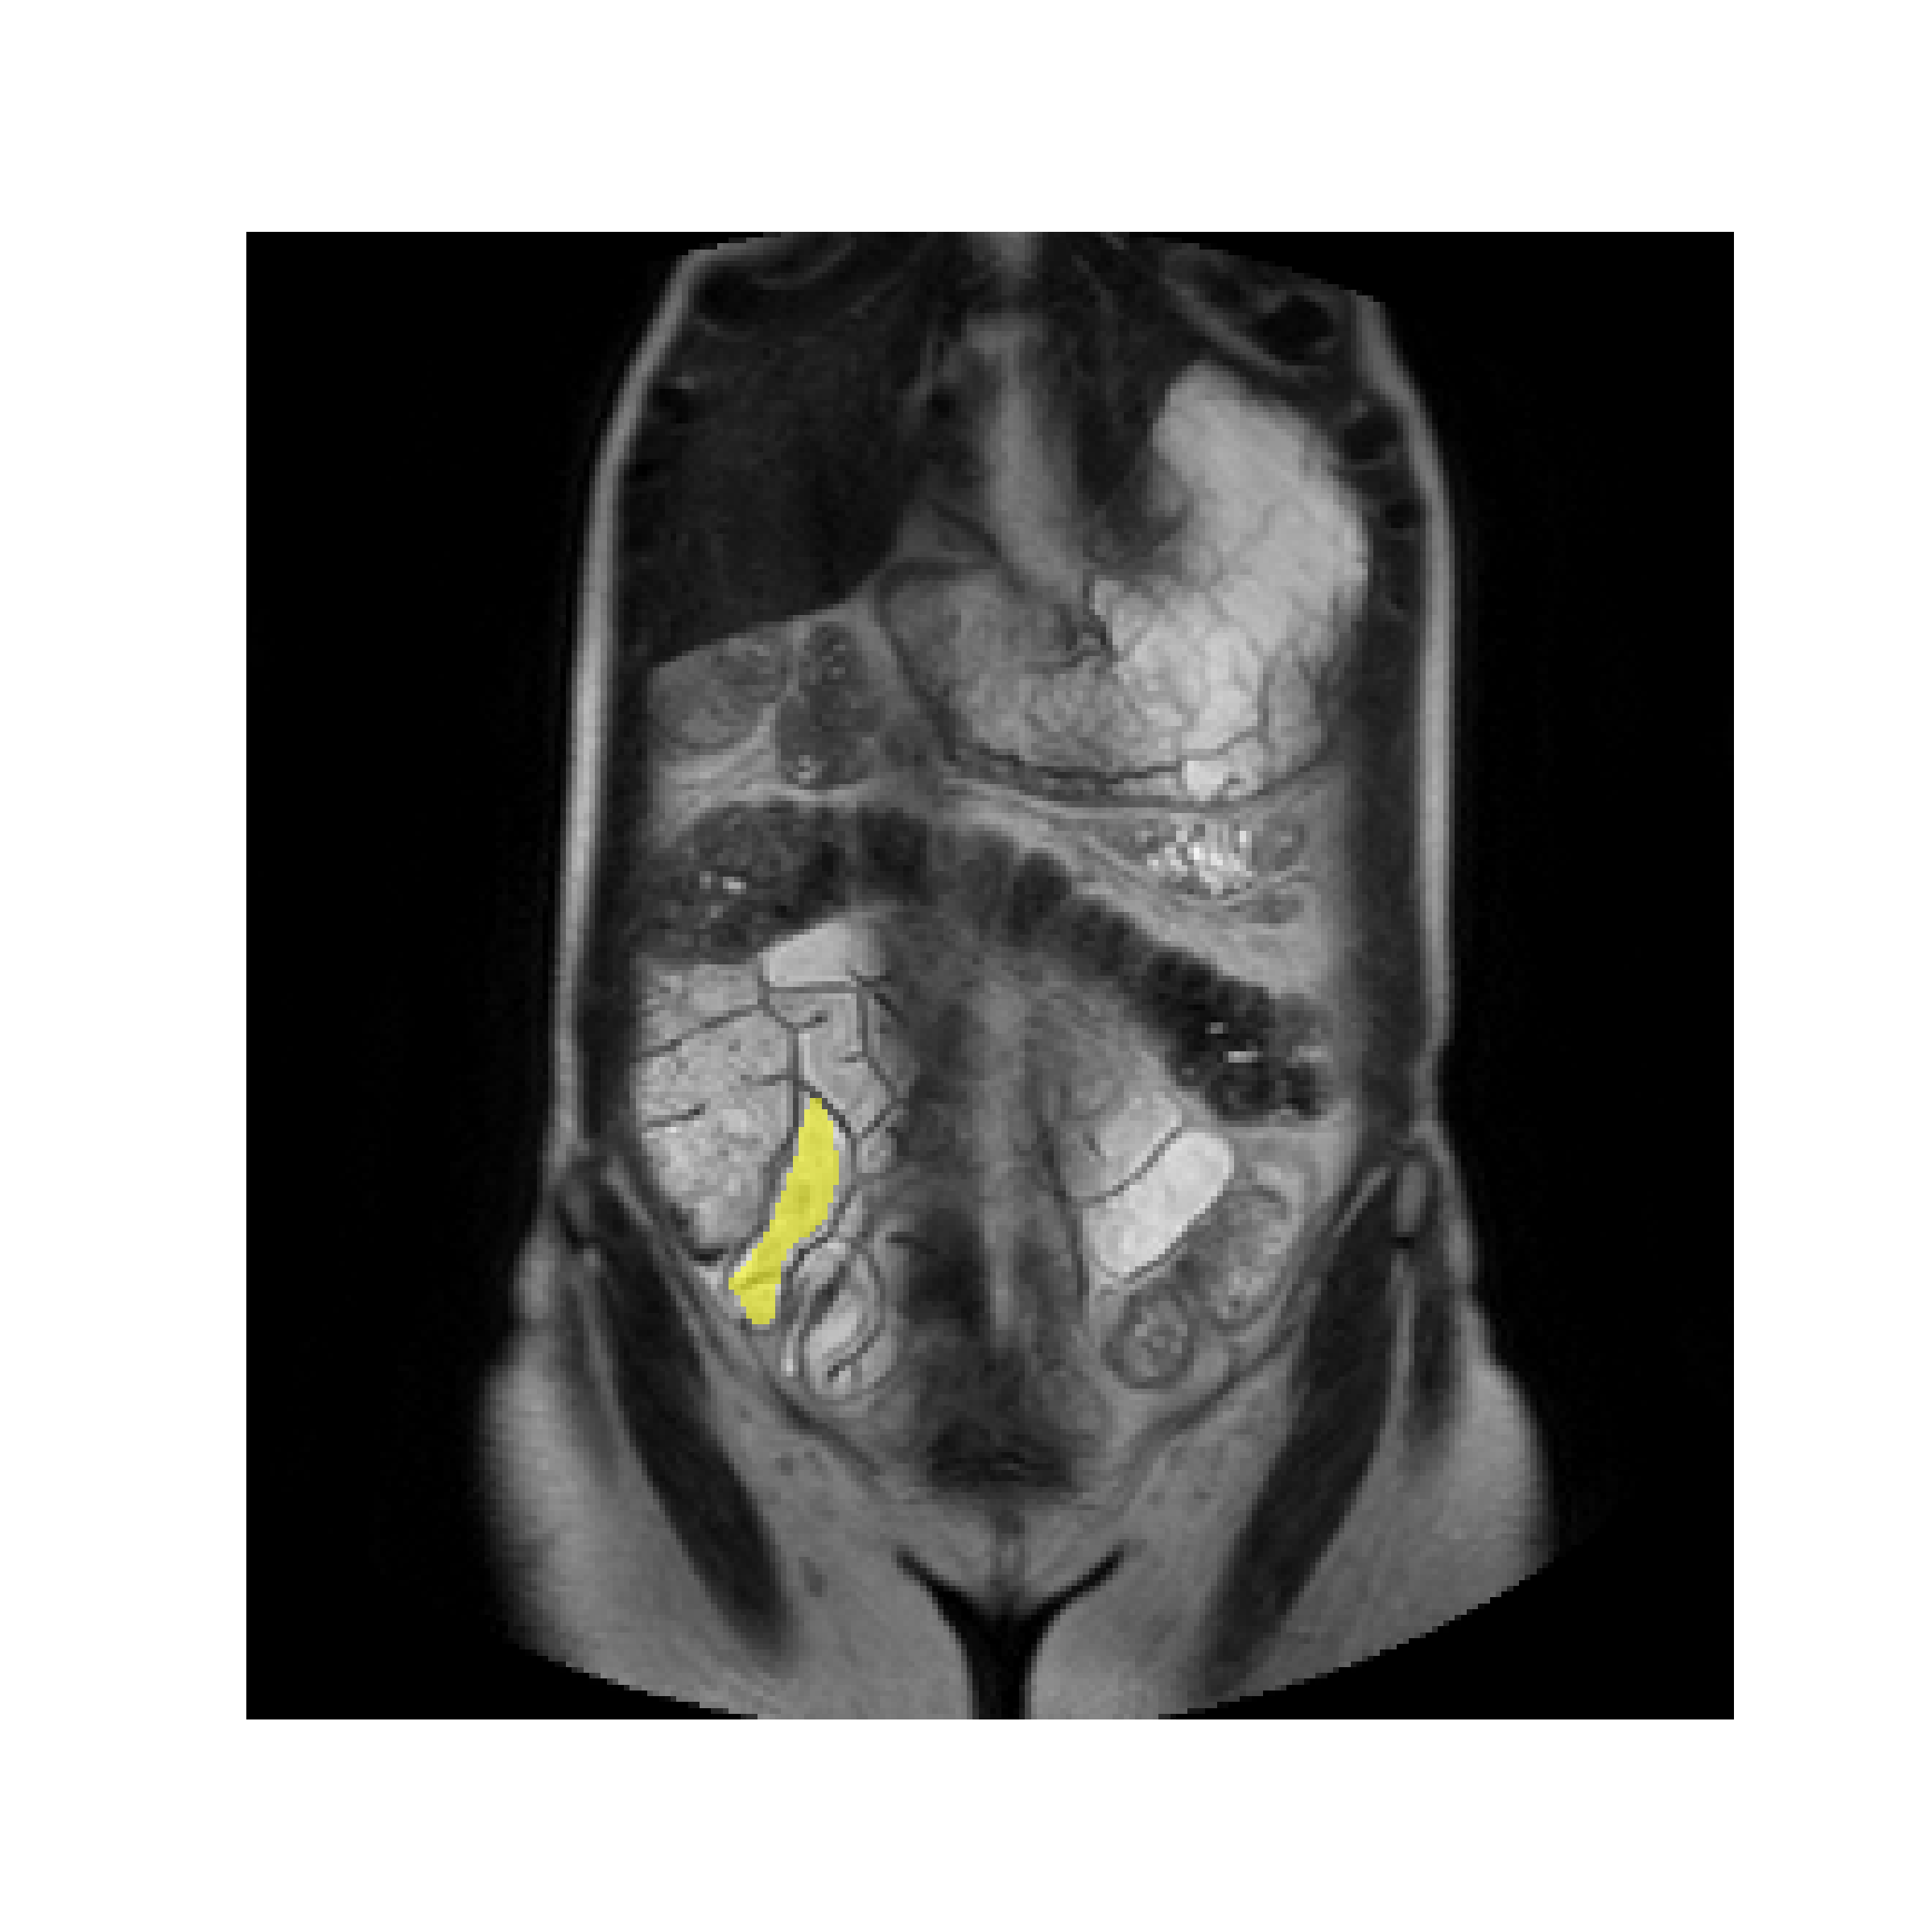
\includegraphics[width=\textwidth]{./figures/weak_mask_coronal_gt.png}
        \caption{Ground Truth on Coronal T2}
        \label{fig:gt-coronal}
    \end{subfigure}
    \hfill
    \begin{subfigure}[b]{0.48\textwidth}
        \centering
        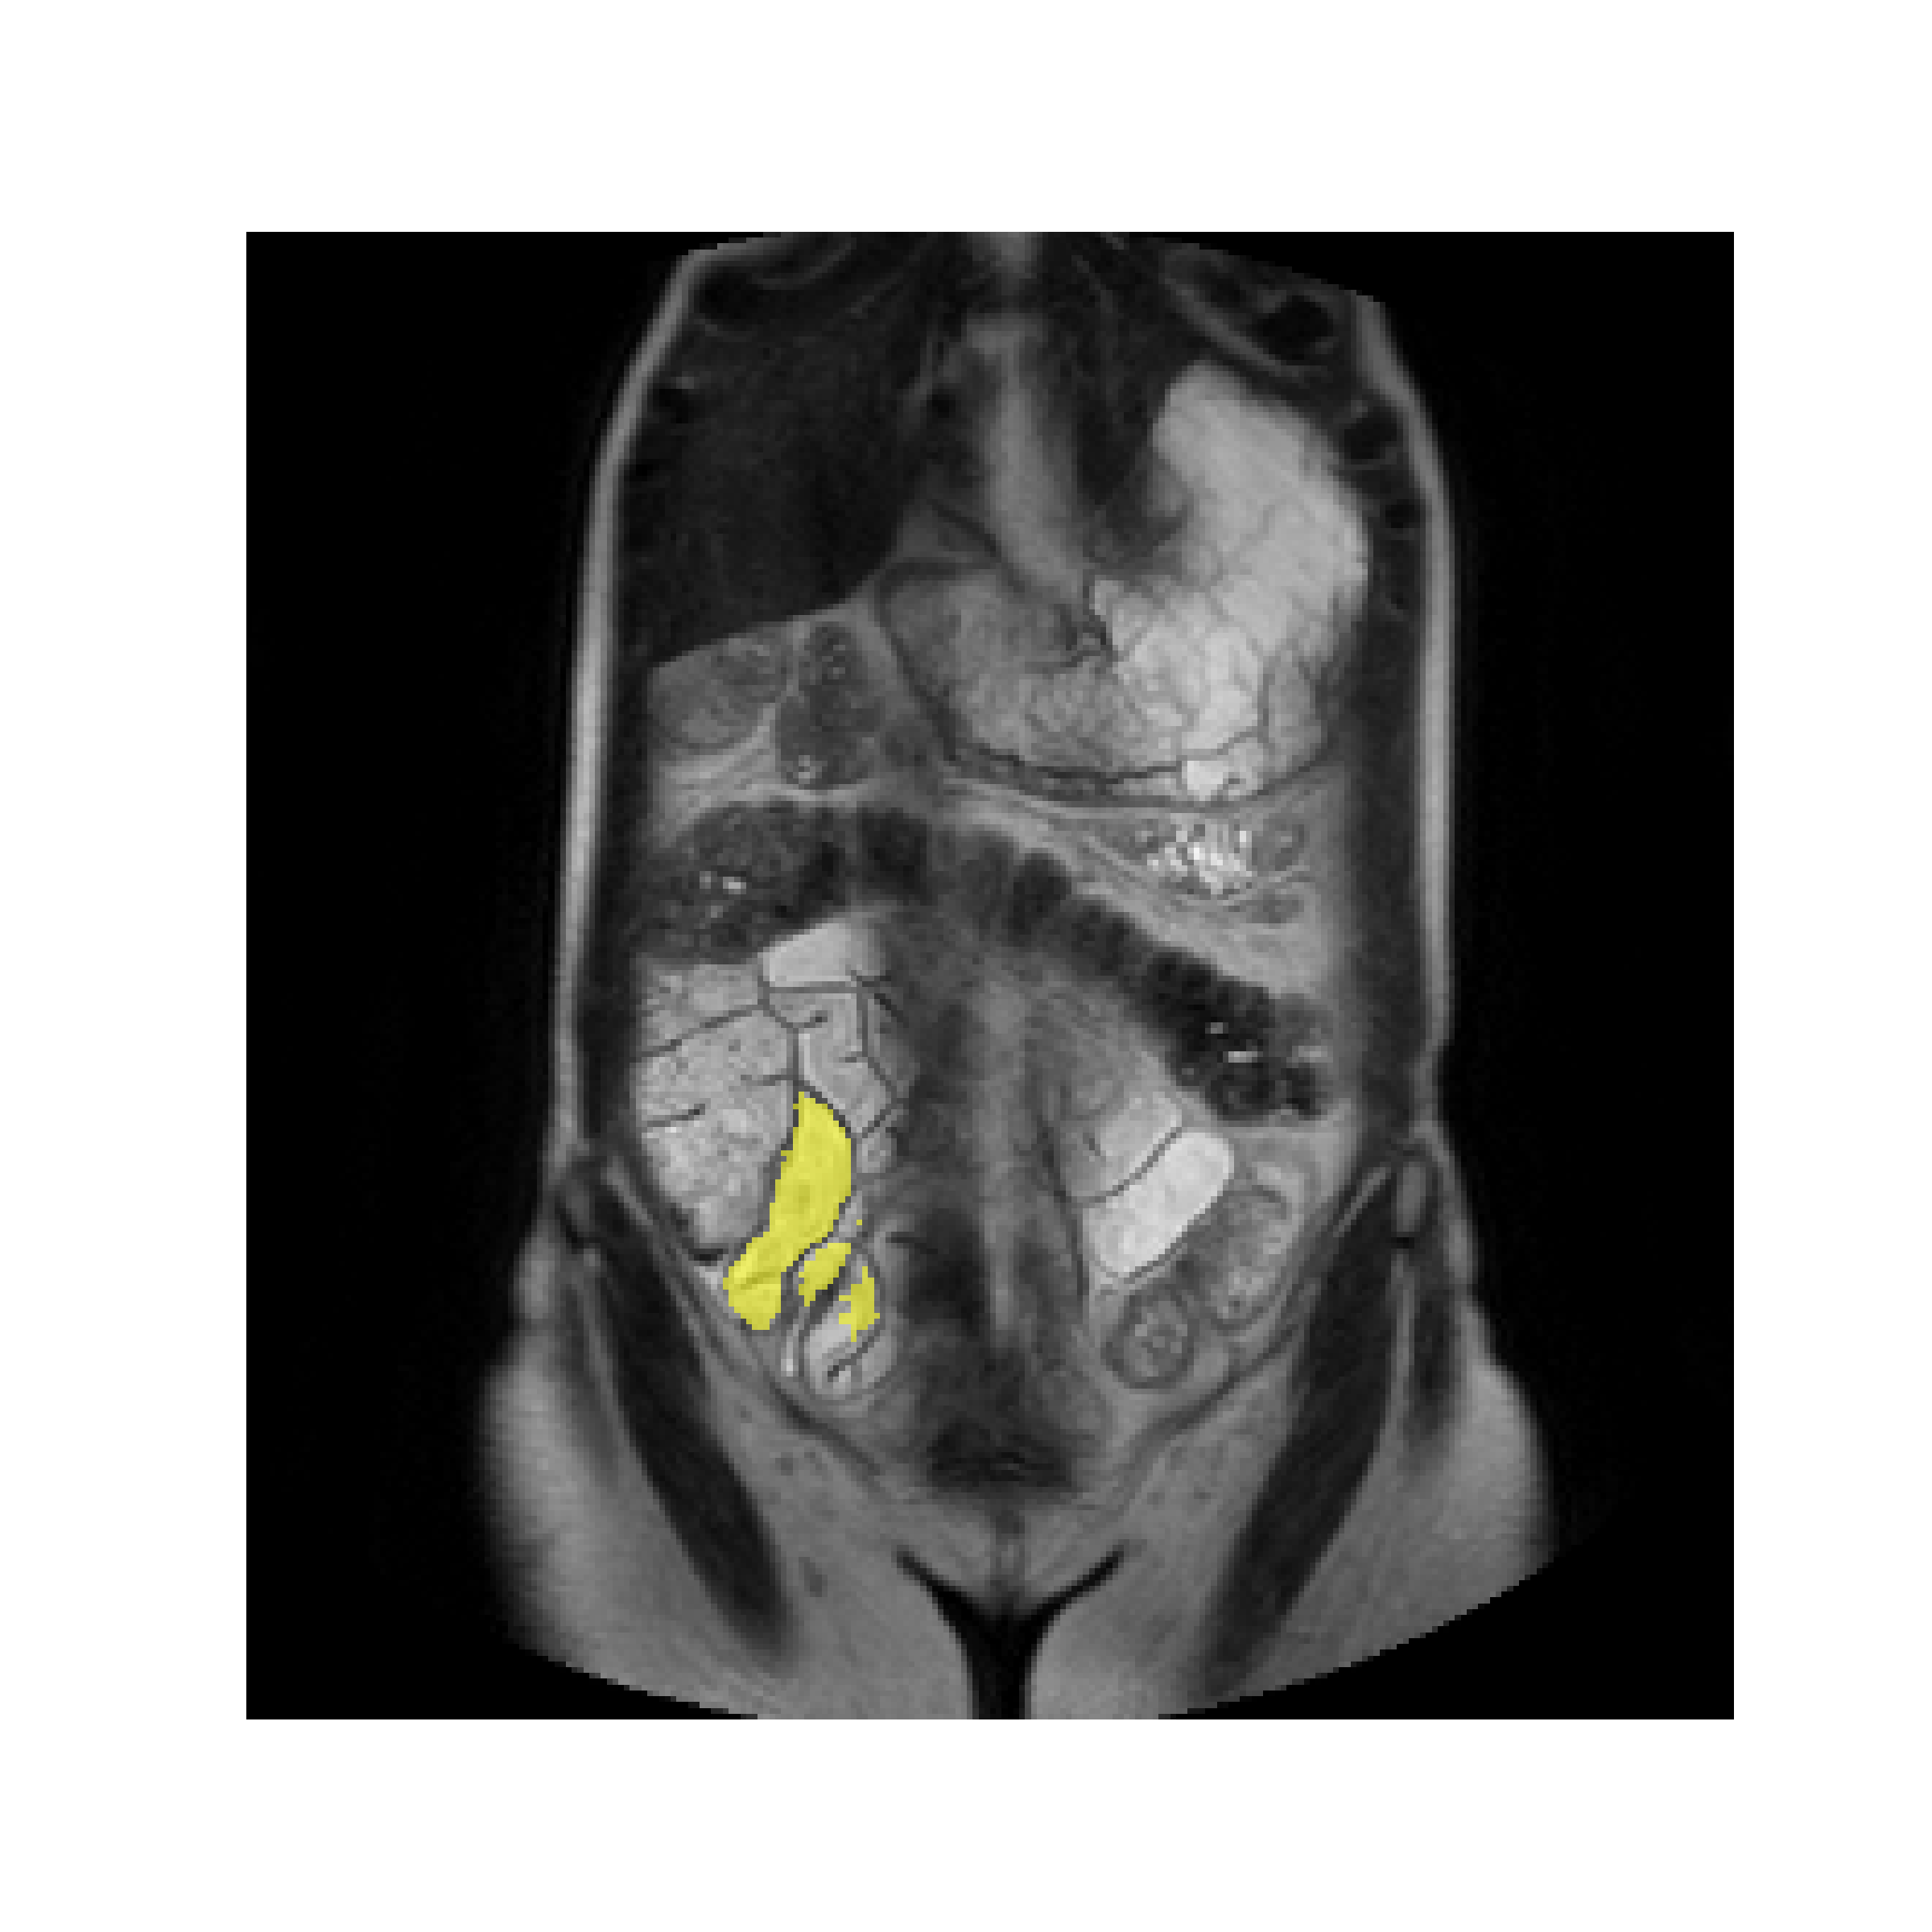
\includegraphics[width=\textwidth]{./figures/weak_mask_coronal_medsam.png}
        \caption{Weak Mask on Coronal T2}
        \label{fig:mask-coronal}
    \end{subfigure}
       \caption{A Cross-Model Comparison between Ground Truth and Generated Weak Masks}
       \label{fig:comparison-mask-gt}
\end{figure}
\subsection{Statistical Evaluation for Establishing Significance}

In a bid to confirm the statistical significance of the enhancements realized through our approach, we employed the two-tailed t-test. Setting a significance level at 0.05, we sought a comparative study across modalities between the baseline and the outcomes generated through our technique.

It is important to note that the t-test utilized is an independent two-sample t-test as it takes into consideration results gathered separately from two distinct groups: the baseline results and those generated by our approach.

The table below presents a detailed view of the t-test outcomes:

\begin{table}[ht]
\centering
\begin{tabular}{c|c|c|c}
Modality & \(t\) statistic & \(p\) value & significance level \\
\hline
Axial & 3.9138 & 0.0029 & 0.05 \\
\hline
Coronal & 2.525 & 0.0355 & 0.05
\end{tabular}
\end{table}

What stands out in these test results is that the \(p\) values for both cases fall below the set significance level. This provides compelling evidence to dismiss our null hypothesis, thereby confirming significant improvements in our weak label generation. Consequently, we can assertively state that our approach tangibly enhances the performances of the processes under study.
\section{Segmentation Model}
similar journey, with t-test
\begin{table}[ht]
    \begin{subtable}[b]{\textwidth}
        \centering
        \begin{tabular}{c | c | c}
        Model & Average DSC (Axial) & Average DSC (Coronal) \\
        \hline
        Baseline & \(0.5785 \pm 0.1742\)  & \(0.5861 \pm 0.1211\)\\
        \hline
        Our Method & \(\mathbf{0.8084 \pm 0.0695}\) & \(\mathbf{0.6931 \pm 0.0724}\) 
       \end{tabular}
       \caption{Average Case Comparison}
       \label{tab:average-sseg}
    \end{subtable}
    \vfill
    \begin{subtable}[b]{\textwidth}
        \centering
        \begin{tabular}{c | c | c}
        Model & Best DSC (Axial) & Best DSC (Coronal) \\
        \hline
        Baseline & 0.6573 & 0.6711\\
        \hline
        Our Method & \(\mathbf{0.8843}\) & \(\mathbf{0.8251}\)
       \end{tabular}
       \caption{Best Case Comparison}
       \label{tab:best-seg}
    \end{subtable}
     \caption{Weak Lable Generation Comparison}
     \label{tab:seg}
\end{table}
\section{Comparison with Ground truth}

\section{Significance}







